\section{VITA-E System Architecture}
\label{sec:architecture}

This section presents the core technical contribution of our work, detailing the architectural and algorithmic innovations that enable flexible and natural human-robot interaction.

\subsection{Overall Framework}

The VITA-E framework is designed around two foundational principles: 1) a \textbf{model-as-controller} paradigm, where a VLM drives system behavior by generating explicit command tokens, and 2) a \textbf{dual-model interaction core} that enables real-time interruption and concurrency.

Our framework adopts a dual-system architecture that has recently become common~\citep{gr00t, pi0}), which consists of a VLM for high-level understanding (System-2) and a diffusion action expert for low-level motor control (System-1). The VLM's primary role is to interpret the user's intent and the scene context, while the action expert translates this understanding into precise physical movements. The logical flow of our approach is illustrated in Figure~\ref{fig:architecture}. It operates primarily in two states: \textbf{Hearing} and \textbf{Action}. In the default \textbf{Hearing} state, the VLM processes image and user language to determine intent. Based on its understanding, it can generate a \texttt{[RES]} token for a purely verbal response, or an \texttt{[ACT]} token, if a physical task is commanded. The generation of this \texttt{[ACT]} token serves as a direct command, transitioning the system into the \textbf{Action} state. In this state, the VLM works with an Action Expert to generate low-level motor commands until the task is finished (signaled by an \texttt{[END]} token) or interrupted by the other model.

This entire logical framework is implemented through a modular server-client implementation, where the server hosts our dual-model core and the client captures the real-world information and executes the action command. The following subsections provide details of: 1) the model-as-controller paradigm enabled by the VLM and its special token-based control language, and 2) the dynamic interaction mechanism enabled by the dual-model core.

\begin{figure*}[!t]
    \centering
    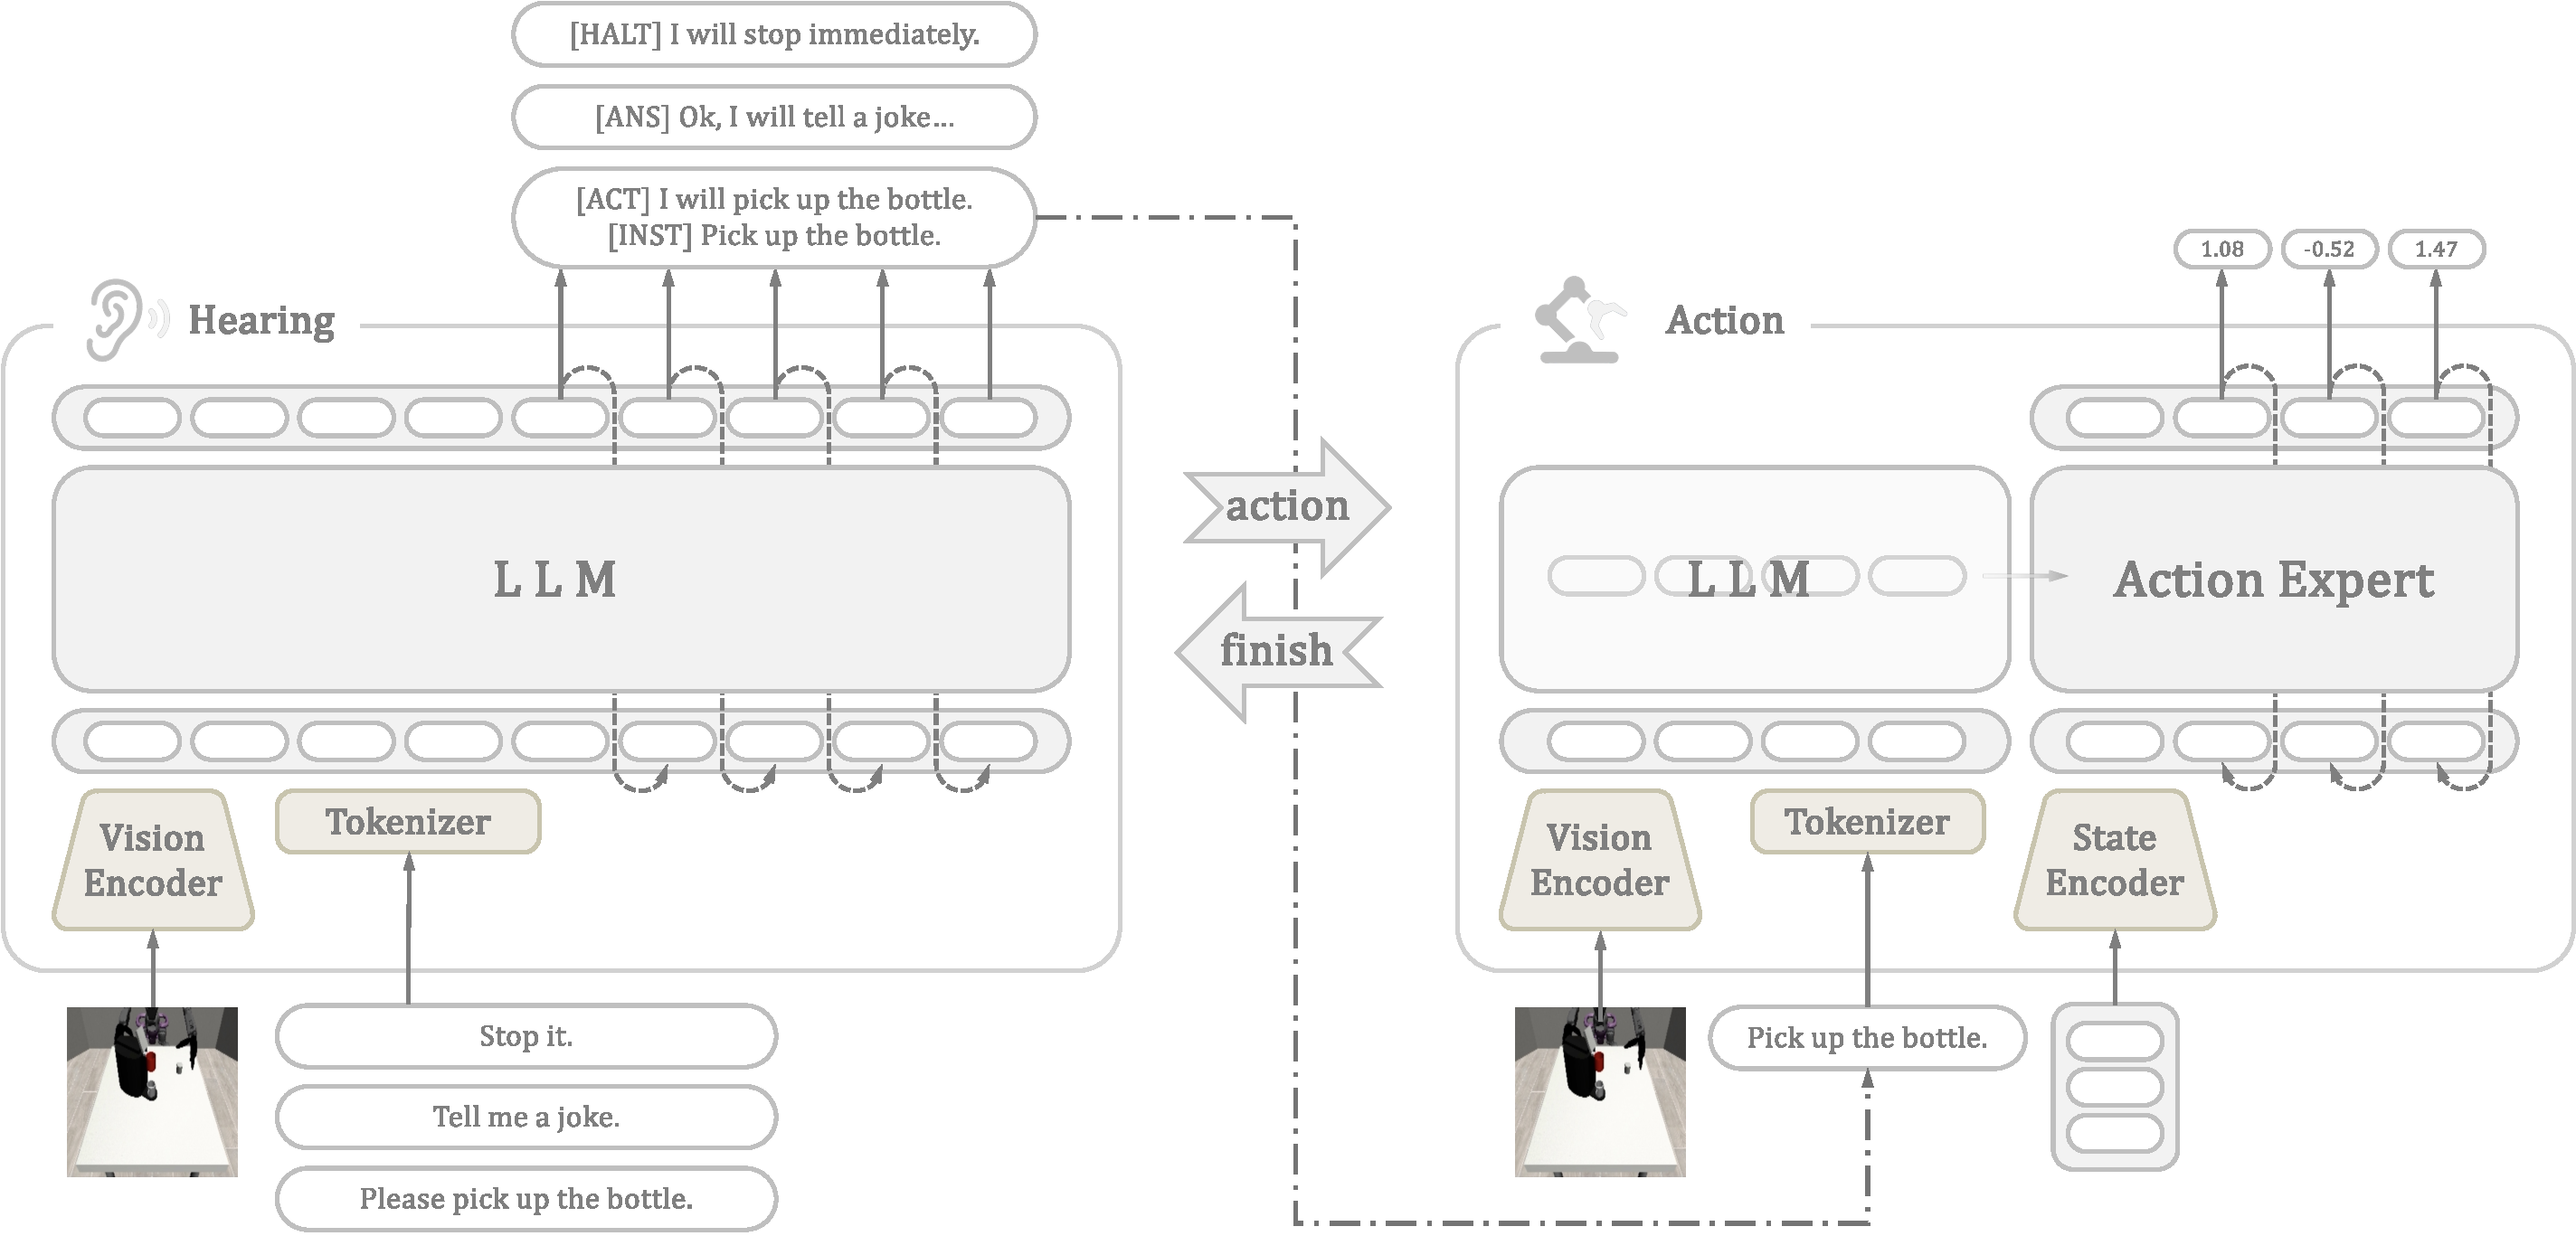
\includegraphics[width=0.8\textwidth]{VITA-E//pic/architecture.pdf}
    \caption{The logical architecture and operational states of the active model in our dual-model VITA-E framework. Each of the two models can switch between ``Active'' and ``Standby'' states. When a model becomes active, the VLM part acts as a controller, processing user inputs in the ``Hearing'' state and generating special tokens that can trigger a transition to the ``Action'' state, where it collaborates with an action expert as a whole VLA model. For example, when the VLM's output starts with the \texttt{[ACT]} token, the text between the \texttt{[ACT]} token and the \texttt{[INST]} token will be played as audio, and the text after the \texttt{[INST]} token will be sent to the VLA model as an action instruction. Otherwise, the text after the special token will only be played as audio, and the system will execute the command corresponding to the special token. For the detailed functions of each special token, see Table~\ref{tab:special-token-details}.}
    \label{fig:architecture}
    \vspace{-2em}
\end{figure*}

\subsection{The Model-as-Controller Paradigm}

\subsubsection{Problem Formulation}

The goal of our framework is to learn a policy that maps the current sensory inputs and user instructions to a sequence of robot actions, while also generating verbal responses concurrently and handling interruptions dynamically. Formally, at each timestep $t$, the system receives a visual input $I_t$, the robot's proprioceptive state $q_t$, and a natural language instruction from the user $L_t^{\text{user}}$. The objective is to produce a verbal response  $L_t^{\text{robot}}$ for the user, a system behavior control $c_t$, and a corresponding action chunk $A_t$ for the robot to execute.

\subsubsection{The Control Language: VLM with Special Tokens}

Our key innovation is to have the VLM produce not only semantic understanding but also explicit system-level commands via a learned “control language.” The VLM, denoted as $\pi_{\text{VLM}}$, consumes the visual input $I_t$ and user instruction $L_t^{\text{user}}$ and outputs a structured string $S_t=(c_t, L_t^{\text{robot}}, C_t^{\text{robot}})$. Here, $c_t$ is a discrete control token (see Table~\ref{tab:special-token-details}), $L_t^{\text{robot}}$ is the verbal response, and $C_t^{\text{robot}}$ is an action command that is absent ($\varnothing$) unless $c_t$ indicates that robot action is required. The VLM is trained to learn $\pi_{\text{VLM}}(S_t \mid I_t, L_t^{\text{user}})$.

\begin{table}[thb!]
    \caption{Special tokens used to control the VITA-E framework's behavior.}
    \label{tab:special-token-details}
    \centering
    \resizebox{\linewidth}{!}{%
    \begin{tabular}{@{}lp{5.5cm}p{5cm}@{}}
    \toprule
    \textbf{Token} & \textbf{Description} & \textbf{Example Model Output} \\ \midrule
    \texttt{[RES]} & Signals a voice-only response. Generated as the first token for conversational replies. & \texttt{[RES]} I see an apple on the table. \\
    \addlinespace
    \texttt{[ACT]} & Signals that the response includes a physical action. Generated as the first token to enter action mode.
    & \multirow{2}{*}{\parbox{5cm} {\texttt{[ACT]} Okay, I will put the toy in the box. \texttt{[INST]} Pick up toy and place in box.}} \\
    \addlinespace
    \texttt{[INST]} & Delimits the spoken part of an action response from the internal action instruction that follows. \\
    \addlinespace
    \texttt{[HALT]} & Commands an immediate stop of the current action. Generated as the first token for emergency stops. & \texttt{[HALT]} Stopping immediately. \\
    \addlinespace
    \texttt{[END]} & Signals that a multi-step action sequence has been successfully completed. & \texttt{[END]} The action is finished. \\ \bottomrule
    \end{tabular}%
    }
\end{table}

Teaching the VLM to generate these control tokens required a specialized data curation process that goes beyond standard instruction-following datasets. We reformat and synthetically augment the embodied scenario vision-language data to explicitly teach the VLM to output control tokens as desired, based on datasets including ActionNet~\citep{fourier2025actionnet}, Libero~\citep{liu2023libero}, and self-collected real-world scenario data.

The process is as follows: we first process our aggregated dataset of demonstration trajectories, which initially consists of video, instructions, and actions. We then apply an automated annotation pipeline to insert the special tokens into the target output based on the context of each trajectory:
\begin{itemize}
    \item For trajectories where the instruction is a question (e.g., ``What do you see?'') and no significant action occurs, the target response is prepended with the \texttt{[RES]} token.
    \item For trajectories involving physical manipulation, the target response is prepended with \texttt{[ACT]}. A spoken confirmation (e.g., ``Okay, I'll do that.'') is generated, followed by the \texttt{[INST]} token and the cleaned original task instruction.
    \item To create training instances for interruption, we take an existing action trajectory and inject a new user input like ``Stop!'' at a random point. The corresponding target output for this synthetic data point is then formulated as ``\texttt{[HALT]} Okay, stopping.''.
    % This crucial step allows the model to learn to respond to interruptions, a scenario rarely captured in standard teleoperation datasets.
    \item Finally, to teach the model to signal task completion, we use the final state of successful trajectories. At the point where the task is complete and after, we create training instances where the target output begins with a special \texttt{[END]} token.
    % During inference, each forward pass of the model within the action loop generates a sequence of tokens. The framework inspects the first of these tokens; if it is decoded as \texttt{[END]}, the system terminates the action loop, thereby finishing the entire task.
\end{itemize}
This data curation strategy transforms the fine-tuning task. Instead of merely learning to describe or plan actions, the VLM learns to output a structured string that simultaneously contains a conversational reply, a system-level command (the special token), and a semantic goal for the action expert. This approach is what enables the tight coupling between high-level reasoning and low-level system execution that defines our framework.

\subsubsection{Action Expert for Motor Control}
The action expert can be denoted as $\pi_a$, and the generation process of the action chunk will be $A_t = \pi_a(h_t, q_t)$, where $h_t = \pi_{\text{VLM}}(I_t, C_t^{\text{robot}})_{\text{hidden}}$ is the hidden states of the VLM. We adopt the Diffusion Transformer from GR00T~\citep{gr00t} as $\pi_a$, which has been pre-trained on large-scale embodied data, providing a strong foundation for motor control. Following our two-stage training paradigm, we further fine-tune this model on task-specific data collected from our target robot. During this stage, we exclusively train the projection head. This approach adapts the model to the specific kinematics of our robot while preventing overfitting. The action expert is trained to predict a sequence of robot joint angles, translating the VLM's high-level semantic goal into low-level, executable trajectories.

\subsection{Dynamic Interaction via a Dual-Model Architecture}

The core of VITA-E's interactivity lies in its unique dual-model architecture, a design inspired by the cooperative mechanism of the brain's hemispheres. This ``two hemispheres'' approach allows one model instance---the \textbf{Active Model}---to remain focused on executing the current task, while the other instance---the \textbf{Standby Model}---serves as an observer. This structure enables the robot to instantly shift its attention to achieve flexible concurrency and seamless interruptions. The coordination between these two hemispheres is managed by synchronization primitives (e.g., semaphores) that control which model is active and, crucially, grant the Standby Model the authority to intervene in its counterpart. The four primary interaction patterns that emerge from this architecture are illustrated in Figure~\ref{fig:logic}.

\begin{figure*}[t!]
    \centering
    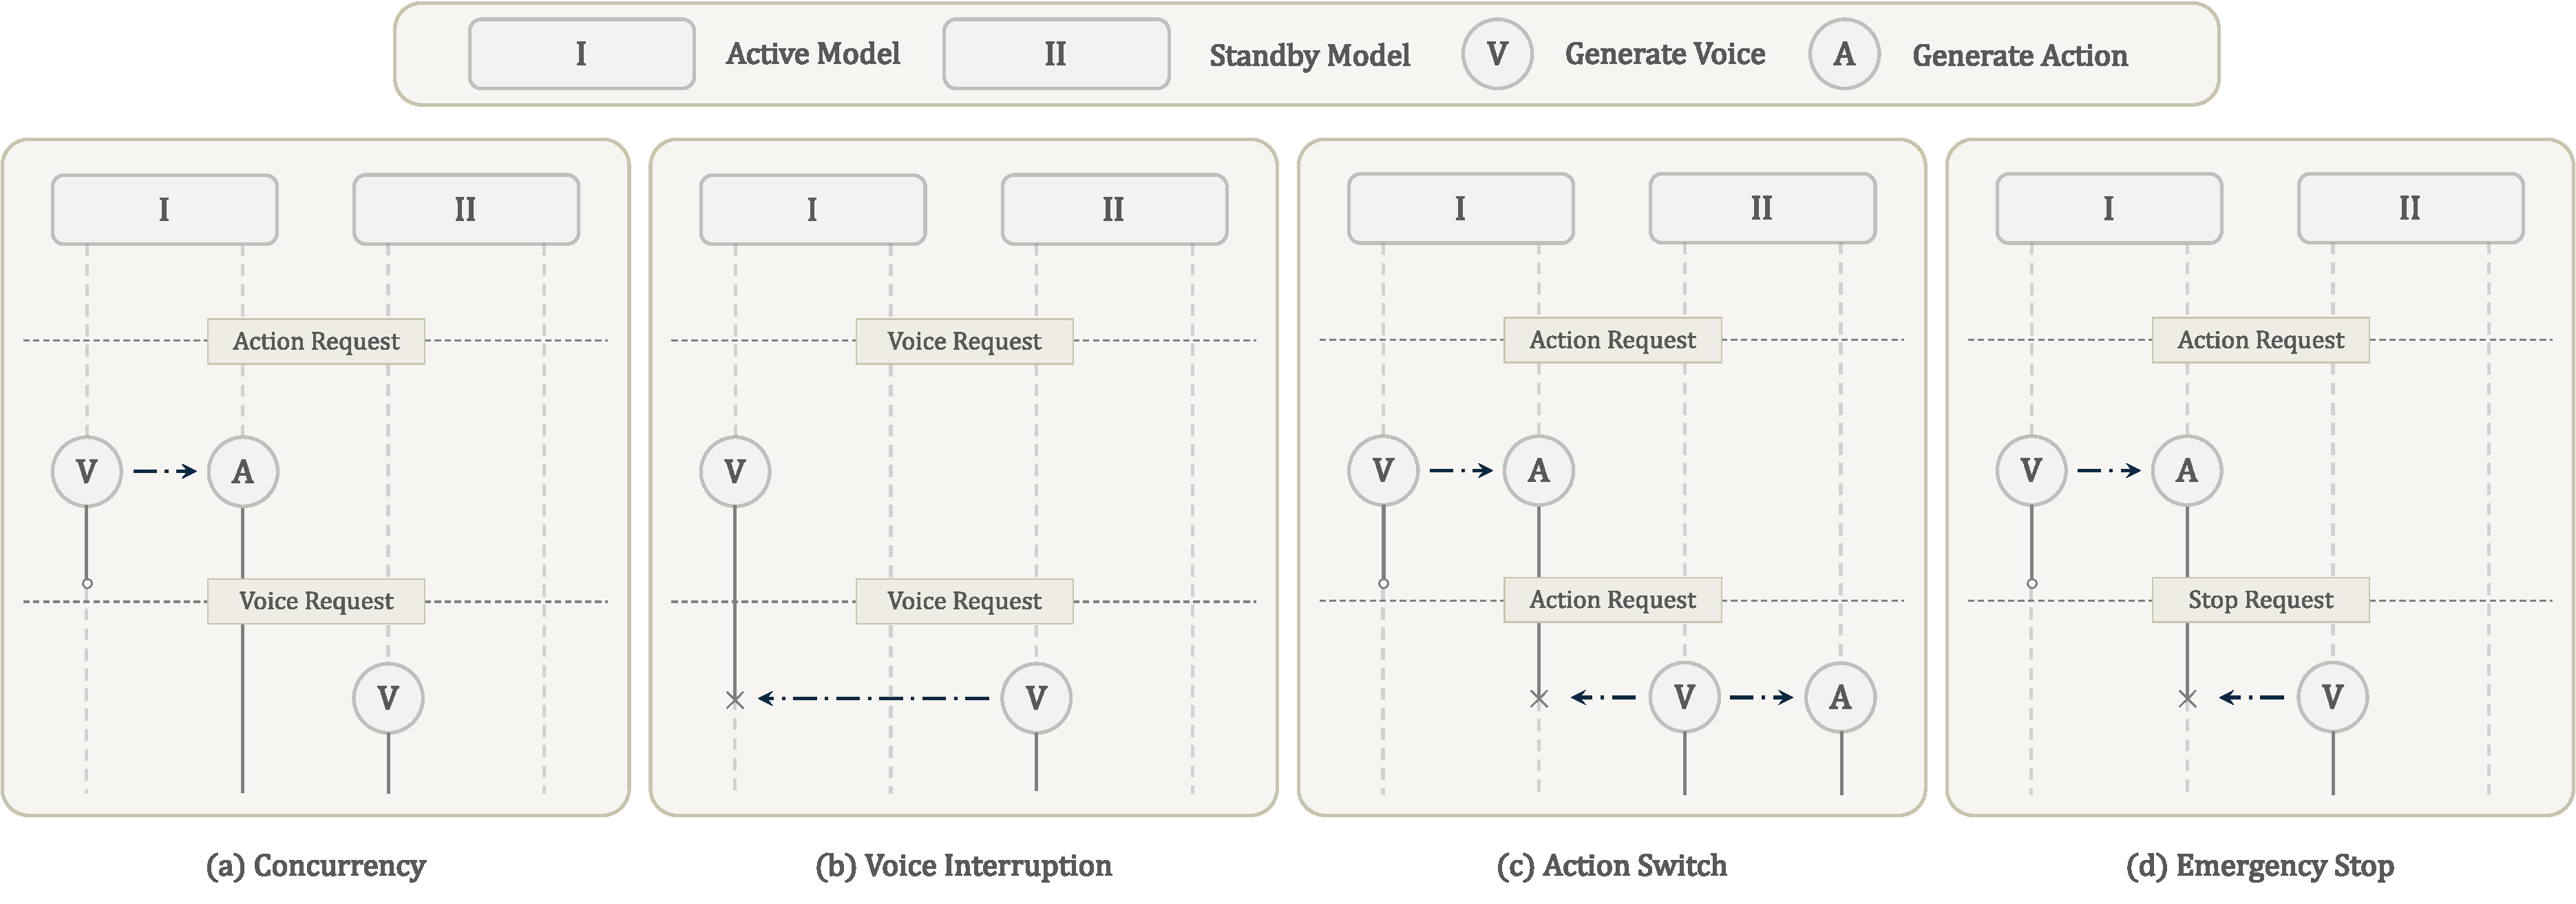
\includegraphics[width=\textwidth]{VITA-E//pic/logic.pdf}
    \caption{Sequence diagrams illustrating the four primary interaction modes. Model I is the Active Model, and Model II is the Standby Model. V and A represent voice and action generation, respectively. The Standby Model can process new requests in parallel or preempt the Active Model to handle interruptions and task switches.}
    \label{fig:logic}
    \vspace{-2em}
\end{figure*}

\textbf{Concurrency}
VITA-E is able to perform physical actions and speak simultaneously, as depicted in Figure~\ref{fig:logic}(a). When the Active Model (I) is engaged in an \texttt{Action Request}, it enters a protected state. If a new \texttt{Voice Request} arrives, the Standby Model (II) assesses the Active Model's state. Recognizing that an action is in progress, it proceeds to handle the conversational query independently by generating its own voice response, all without interrupting the ongoing physical task. This allows the robot to answer questions while continuing its work.

\textbf{Voice Interruption}
As shown in Figure~\ref{fig:logic}(b), the framework allows users to interrupt the robot's speech at any time. While the Active Model (I) is generating a verbal response to a \texttt{Voice Request}, any subsequent input will be routed to the Standby Model (II). The Standby Model's priority is to process this new input: it signals a preemption event that instantly terminates the Active Model's speech generation, ensuring the robot yields to the user for flexible, natural turn-taking.

\textbf{Action Switching}
The framework can dynamically switch from one physical task to another based on user commands, as shown in Figure~\ref{fig:logic}(c). If the Active Model (I) is executing an initial \texttt{Action Request} (Task A), the subsequent new instruction for Task B will be captured by the Standby Model (II). The Standby Model then preempts the Active Model, halting its execution of Task A. Immediately after, the Standby Model becomes the new Active Model and executes Task B. This allows for a seamless switch of the robot's physical behavior. To ensure safety during this transition, a retraction mechanism is employed, which returns the robot to the initial pose by sequentially popping and executing inverse movements from a stored action stack.

\textbf{Emergency Stop}
Another interactive feature is the ability to immediately halt all motion. As illustrated in Figure~\ref{fig:logic} (d), when a user issues a \texttt{Stop Request} while the Active Model (I) is performing an action, the Standby Model (II) processes it with the highest priority. It generates a \texttt{[HALT]} token and triggers an immediate preemption of the Active Model, which breaks its action-generation loop and sends a final halt command to the robot client. This ensures that all physical motion ceases instantly, providing a reliable, highly responsive safety mechanism for the operator.
